
\let\negmedspace\undefined
\let\negthickspace\undefined
\documentclass[journal]{IEEEtran}
\usepackage[a5paper, margin=10mm, onecolumn]{geometry}
%\usepackage{lmodern} % Ensure lmodern is loaded for pdflatex
\usepackage{tfrupee} % Include tfrupee package

\setlength{\headheight}{1cm} % Set the height of the header box
\setlength{\headsep}{0mm}     % Set the distance between the header box and the top of the text

\usepackage{gvv-book}
\usepackage{gvv}
\usepackage{cite}
\usepackage{amsmath,amssymb,amsfonts,amsthm}
\usepackage{algorithmic}
\usepackage{graphicx}
\usepackage{textcomp}
\usepackage{xcolor}
\usepackage{txfonts}
\usepackage{listings}
\usepackage{enumitem}
\usepackage{mathtools}
\usepackage{gensymb}
\usepackage{comment}
\usepackage[breaklinks=true]{hyperref}
\usepackage{tkz-euclide} 
\usepackage{listings}
% \usepackage{gvv}                                        
\def\inputGnumericTable{}                                 
\usepackage[latin1]{inputenc}                                
\usepackage{color}                                            
\usepackage{array}                                            
\usepackage{longtable}                                       
\usepackage{calc}                                             
\usepackage{multirow}                                         
\usepackage{hhline}                                           
\usepackage{ifthen}                                           
\usepackage{lscape}
\begin{document}

\bibliographystyle{IEEEtran}
\vspace{3cm}

\title{4-4.2-17}
\author{EE24BTECH11051 - Prajwal nara
}
% \maketitle
% \newpage
% \bigskip
{\let\newpage\relax\maketitle}

\renewcommand{\thefigure}{\theenumi}
\renewcommand{\thetable}{\theenumi}
\setlength{\intextsep}{10pt} % Space between text and floats


\numberwithin{equation}{enumi}
\numberwithin{figure}{enumi}
\renewcommand{\thetable}{\theenumi}


\textbf{Question}:\\
Find the direction and the normal vector if $y=x+2$
\\ \textbf{Solution: }\\
for $y=mx+c$
    \begin{table}[h!]    
      \centering
      \begin{center}
    \begin{tabular}{|c|c|c|} 
        \hline
            \textbf{Variable} & \textbf{Description} & \textbf{Formula} \\ 
        \hline
            $A$   & It is one end of the line segment & $\myvec{5 \\ -6}$ \\ 
        \hline
            $B$   & It is other end of line segment &  $\myvec{-1\\-4}$\\ 
        \hline
            $C$   & It is the point of intersection of line segment and $Y$-axis & $C  = \myvec{0\\y}$\\ 
        \hline
        
    \end{tabular}
\end{center}  

      \caption{}
    \end{table}\\
Camparing the equation,
\begin{align}
    y=mx+c \ \text{and} \ y=x+2 \\
    m=1 \text \ {and} \ c=2
\end{align}
Hence direction vector is,
\begin{align}
    d = \myvec{1 \\ m}=\myvec{1 \\ 1} 
\end{align}
and normal vector is,
\begin{align}
    n = \myvec{-m \\ 1}=\myvec{-1 \\ 1}
\end{align}

    \begin{figure}[h]
        \centering
       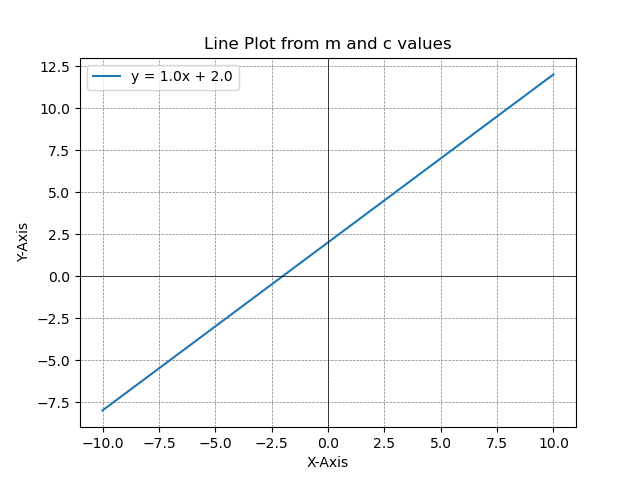
\includegraphics[width=0.7\linewidth]{figs/fig1.png}
       \caption{}
       \label{graph}
    \end{figure}
\end{document}  


